%\pagestyle{plain}

\chapter{Event Detection}
In this chapter, we will introduce the mechanism of event detection in this project. 
We first apply some noise reduction or audio enhancement technique on the training data for our events. 
Then we extract MFCC features from the training clips. 
After getting features, a Gaussian Mixture Model is built on those features. 

\section{Audio Enhancement}
Because the audios downloaded from SSEs are uploaded by other users. 
Those clips are recorded by various types of devices and in different environments. 
Hence we need to apply a noise reduction step to enhance the audio clips. 

Among algorithms for speech enhancement, spectral subtraction was one of the first algorithms proposed. 
Although it was originally proposed for speech enhancement, we use it in our project for noise is pretty much the same in speech or in more general audios. 
The basic principles is that we assume the clean signal add some additive noise becomes the audio we get. 
Then if we subtract the noise spectrum from the audio, we may get signal close to the original clean one. 

Mathematically speaking, assume the input signal is $ y(t) = x(t) + n(t)$, where the signal $x(t)$ is the signal of interest and $n(t)$ is the additive noise. 
The audio enhancement process takes on the following steps:
\begin{enumerate}
\item The input signal $y(t)$ is resampled to 16kHz and multiple channels are averaged to one channel. 
\item Using short time Fourier transform (STFT), we obtain $Y_i(k) = X_i(k) + N_i(k)$, where $i$ is the frame indices and $k$ is the frequency bin indices of the spectrum. 
\item The Minimum Statistics (MS) estimator \cite{martin2001noise} is used to the noise power spectral density from $y(t)$. 
\item Spectral subtraction is used to remove the estimated noice spectrum from the input spectrum $Y_i(k)$. 
Then we could get an estimated clean signal spectrum: $\hat{X_i}(k)$. 
\item Applying inverse short time Fourier transform (ISTFT) on $\hat{X_i}(k)$ to get the estimated clean signal $\hat{x}(t)$. 
\end{enumerate}

A speech processing toolbox for Matlab called VoiceBox is used for spectral subtraction\footnote{\url{http://www.ee.ic.ac.uk/hp/staff/dmb/voicebox/voicebox.html}}.
% noise subtraction example here 

\section{Feature Extraction}
Since the audio data is downloaded from a sound website where clips are crowdsourced, the clips are in various format. 
We converted all audio clips to WAV format and averaged the channels into one if it has multiple channels. 
Moreover, clips are all downsampled to 16khz sample rate for feature extraction. 

For the audio data, mel-frequency cepstrum coefficients (MFCCs) features are a widely-used feature. 
It was brought up by Davis and Mermelstein in the 1980s. 
MFCC features extract the spectral envelope from spectrums of audio frames.
Basically, the process of extracting MFCCs start by applying Fast Fourier transform (FFT) on framed audio. 
FFT transform audio data from Amplitude-Time domain (frame) into Amplitude-Frequency domain (spectrum).  
As each audio frame is transformed into a spectrum, the spectral envelope is extracted by Inverse FFT (IFFT).

Actually, one more filtering is performed before applying IFFT on spectrums. 
Because MFCC features are based on human perceptual experiment, and human's ear is like a natural filter, where low-frequency area has more filter and high-frequency area has less. So a nonlinear function is applied to original spectrum to transform the frequency axis into the mel scale. 
A popular formula to convert $f$ herts into $m$ mel is:  
\begin{equation}
	m = 2595 \times \log_{10}(1+\frac{1}{700})
\end{equation} 

% melscale.eps on 5566
\begin{figure}[htb]
\centering
% GNUPLOT: LaTeX picture with Postscript
\begingroup
  \makeatletter
  \providecommand\color[2][]{%
    \GenericError{(gnuplot) \space\space\space\@spaces}{%
      Package color not loaded in conjunction with
      terminal option `colourtext'%
    }{See the gnuplot documentation for explanation.%
    }{Either use 'blacktext' in gnuplot or load the package
      color.sty in LaTeX.}%
    \renewcommand\color[2][]{}%
  }%
  \providecommand\includegraphics[2][]{%
    \GenericError{(gnuplot) \space\space\space\@spaces}{%
      Package graphicx or graphics not loaded%
    }{See the gnuplot documentation for explanation.%
    }{The gnuplot epslatex terminal needs graphicx.sty or graphics.sty.}%
    \renewcommand\includegraphics[2][]{}%
  }%
  \providecommand\rotatebox[2]{#2}%
  \@ifundefined{ifGPcolor}{%
    \newif\ifGPcolor
    \GPcolorfalse
  }{}%
  \@ifundefined{ifGPblacktext}{%
    \newif\ifGPblacktext
    \GPblacktexttrue
  }{}%
  % define a \g@addto@macro without @ in the name:
  \let\gplgaddtomacro\g@addto@macro
  % define empty templates for all commands taking text:
  \gdef\gplbacktext{}%
  \gdef\gplfronttext{}%
  \makeatother
  \ifGPblacktext
    % no textcolor at all
    \def\colorrgb#1{}%
    \def\colorgray#1{}%
  \else
    % gray or color?
    \ifGPcolor
      \def\colorrgb#1{\color[rgb]{#1}}%
      \def\colorgray#1{\color[gray]{#1}}%
      \expandafter\def\csname LTw\endcsname{\color{white}}%
      \expandafter\def\csname LTb\endcsname{\color{black}}%
      \expandafter\def\csname LTa\endcsname{\color{black}}%
      \expandafter\def\csname LT0\endcsname{\color[rgb]{1,0,0}}%
      \expandafter\def\csname LT1\endcsname{\color[rgb]{0,1,0}}%
      \expandafter\def\csname LT2\endcsname{\color[rgb]{0,0,1}}%
      \expandafter\def\csname LT3\endcsname{\color[rgb]{1,0,1}}%
      \expandafter\def\csname LT4\endcsname{\color[rgb]{0,1,1}}%
      \expandafter\def\csname LT5\endcsname{\color[rgb]{1,1,0}}%
      \expandafter\def\csname LT6\endcsname{\color[rgb]{0,0,0}}%
      \expandafter\def\csname LT7\endcsname{\color[rgb]{1,0.3,0}}%
      \expandafter\def\csname LT8\endcsname{\color[rgb]{0.5,0.5,0.5}}%
    \else
      % gray
      \def\colorrgb#1{\color{black}}%
      \def\colorgray#1{\color[gray]{#1}}%
      \expandafter\def\csname LTw\endcsname{\color{white}}%
      \expandafter\def\csname LTb\endcsname{\color{black}}%
      \expandafter\def\csname LTa\endcsname{\color{black}}%
      \expandafter\def\csname LT0\endcsname{\color{black}}%
      \expandafter\def\csname LT1\endcsname{\color{black}}%
      \expandafter\def\csname LT2\endcsname{\color{black}}%
      \expandafter\def\csname LT3\endcsname{\color{black}}%
      \expandafter\def\csname LT4\endcsname{\color{black}}%
      \expandafter\def\csname LT5\endcsname{\color{black}}%
      \expandafter\def\csname LT6\endcsname{\color{black}}%
      \expandafter\def\csname LT7\endcsname{\color{black}}%
      \expandafter\def\csname LT8\endcsname{\color{black}}%
    \fi
  \fi
  \setlength{\unitlength}{0.0500bp}%
  \begin{picture}(7200.00,5040.00)%
    \gplgaddtomacro\gplbacktext{%
      \csname LTb\endcsname%
      \put(858,440){\makebox(0,0)[r]{\strut{} 0}}%
      \csname LTb\endcsname%
      \put(858,1059){\makebox(0,0)[r]{\strut{} 500}}%
      \csname LTb\endcsname%
      \put(858,1679){\makebox(0,0)[r]{\strut{} 1000}}%
      \csname LTb\endcsname%
      \put(858,2298){\makebox(0,0)[r]{\strut{} 1500}}%
      \csname LTb\endcsname%
      \put(858,2917){\makebox(0,0)[r]{\strut{} 2000}}%
      \csname LTb\endcsname%
      \put(858,3536){\makebox(0,0)[r]{\strut{} 2500}}%
      \csname LTb\endcsname%
      \put(858,4156){\makebox(0,0)[r]{\strut{} 3000}}%
      \csname LTb\endcsname%
      \put(858,4775){\makebox(0,0)[r]{\strut{} 3500}}%
      \csname LTb\endcsname%
      \put(990,220){\makebox(0,0){\strut{} 0}}%
      \csname LTb\endcsname%
      \put(2153,220){\makebox(0,0){\strut{} 2000}}%
      \csname LTb\endcsname%
      \put(3315,220){\makebox(0,0){\strut{} 4000}}%
      \csname LTb\endcsname%
      \put(4478,220){\makebox(0,0){\strut{} 6000}}%
      \csname LTb\endcsname%
      \put(5640,220){\makebox(0,0){\strut{} 8000}}%
      \csname LTb\endcsname%
      \put(6803,220){\makebox(0,0){\strut{} 10000}}%
    }%
    \gplgaddtomacro\gplfronttext{%
    }%
    \gplbacktext
    \put(0,0){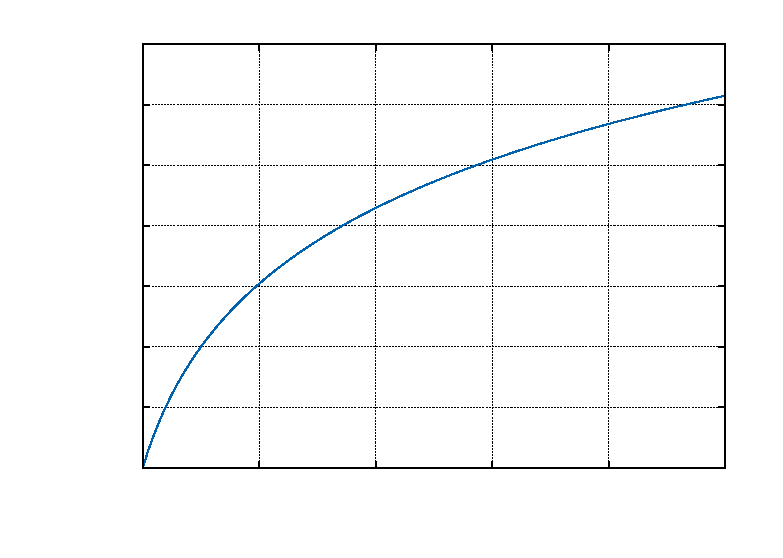
\includegraphics{melscale}}%
    \gplfronttext
  \end{picture}%
\endgroup

\caption{Mel scale versus hertz scale}
\label{fig:melscale}
\end{figure}

Figure \ref{fig:melscale} shows the non-linear transformation of hertz scale to mel scale. 
We could see that the slope of the curve are decreasing as the pitch goes up in hertz scale. 
Because of this feature of suppressing the higher frequency bands, MFCC enables a focus of the more useful range of bands in lower scale \cite{davis1980comparison}.

% Paraphrase !!!

\section{Model Selection}
From the previous feature extraction process, we could a matrix representation for an audio clip. 
The column number stands for the dimension of the features and each row corresponds to one observation. 
From these data, we need to build a model that can capture the overall feature distribution and also are convenient to use for testing data.

For this goal, Gaussian Mixture Model (GMM) is used. 
First, a multivariate gaussian distribution has the following probability density:

% multivariate gaussian 
\begin{equation}
 \mathcal{N}(\mathbf{x}| \mathbf{\mu}, \Sigma) = 
\frac{1}{\sqrt{(2\pi)^D|\Sigma|}}e^{-\frac{1}{2}(\mathbf{x}-\mathbf{\mu})^T \Sigma^{-1} (\mathbf{x}-\mathbf{\mu})}
\end{equation}

In this equation, $\mathbf{\mu}$ and $\mathbf{\Sigma}$ are all vectors in $D$ dimensions, for discribing high dimensional data. 
A gaussian mixture model (or density) is a weighted sum of N gaussian densities. 
Typically, these gaussian densities have the same dimension, say $D$, and each gaussian are called a component.  
Put many gaussian distributions together, we could get the density function for GMM: 

% GMM density function
\begin{equation}
P(\mathbf{x}|\mathbf{\pi},\mathbf{\mu},\Sigma) = \sum_{k = 1}^{M} \pi_k
\mathcal{N}(\mathbf{x}|\mathbf{\mu}_k, \Sigma_k),
\end{equation} 

The intuition of using GMM to model the audio events is that the individual component densities of a multi-model density may model some underlysing set of acoustic classes \cite{reynolds1995robust}. 
Like in speech, a words may consist of some vowels and consonants. 
An audio event is naturally more complicated than speech, and may therefore contain more characteristics. 
Therefore, we use different gaussian densities with different $\mathbf{\mu}$ and $\mathbf\sigma$, where the $\mathbf\mu$ may capture the overall value for one class and the $\mathbf\sigma$ shows the variation of that class.  
When these densities are added together, forming a GMM, they can have a good depiction of some unusual distributions. 

%Before training GMMs for event training data, we first apply K-means algorithm on the data. 
%K-means is also an unsupervised clustering method. 
%It uses a Expectation-Maximization step to update the cluster centroid. 
%Because K-means has a faster speed for iterating than GMMs, so we first run K-means and use its centroid result as initials for further iterating of GMMs. 
%This part use the gaussian toolbox provided by Matlab\footnote{\url{http://cn.mathworks.com/help/stats/gmdistribution-class.html}} . 


\section{Training Data Selection}
As previously mentioned, many of the clips in those Sound Search Engines are crowdsourced. 
Hence, the quality of those clips are not guaranteed to be suitable as our event training data.    
We need to select out those data which are similar, and discard those outliers. 
Because outliers are very likely to be a noise, thus adding no knowledge for our event models, perhaps even bring bad effects. 

Therefore, in our project, we added a step for comparing the similarity of the audio clips, and cluster similar clips together, while leaving others clips out. 
Yet signal data of the audio clips are in different volume, and different duration, it is hard to directly compare their similarity. 
So we resort to the distance between their corresponding GMMs. 
Because the trained GMM are in the same dimension for different audio clips, and GMM represent the overall features, it is reasonable to cluster similar GMMs together. 

In order to measure the distance between GMMs, we use Kullback-Leibler (KL) divergence. 
KL divergence is a measure of the difference between two probability distributions. 
More precisely, KL divergence of $Q$ from $P$, denoted by $KL(P||Q)$, is a measure of the information loss when we use $Q$ to approximate $P$.

For continuous random variables $\mathbf{x}$ and two distributions $P$ and $Q$, the KL divergence of $Q$ from $P$ is defined as:
\begin{equation}
KL(P||Q) = \int_{-\infty}^{+\infty}\ln(\frac{p(\mathbf{x})}{q(\mathbf{x})})p(\mathbf{x})\mathrm{d}x,
\label{eq:kl}
\end{equation}
where $p(\mathbf{x})$ and $q(\mathbf{x})$ are the density functions of $P$ and $Q$.
The divergence satisifies three properties: 
\begin{enumerate}
\item{Self similarity: $KL(P||P) = 0$}. 
\item{Self identification: $KL(P||Q) = 0$, only if $P = Q$}. 
\item{Non-Negativity: $KL(P||Q) >= 0$ for any $P, Q$}. 
\end{enumerate}

Because of these properties, KL divergence is used in many aspects of speech recognition \cite{olsen2003efficient}. 
But we need to take notice that KL divergence is not a distance because it is not symmetric: $KL(P||Q) \neq KL(Q||P)$. 
For two gaussian distributions, the KL divergence has a closed formed expression. 
But for two gaussian mixture models, there is no such closed form expression. 
To tackle this issue, we use an approximation method to the KL divergence proposed in \cite{hershey2007approximating}
It uses ``variational approximation'' for calculating KL divergence. 
We use the \textit{gaussmixk} function in VoiceBox toolbox for implementing the approximated KL divergence\footnote{\url{http://www.ee.ic.ac.uk/hp/staff/dmb/voicebox/doc/voicebox/gaussmixk.html}}. 

\section{Summary}
The method we propose for audible event detection are introduced in this chapter. 
We first apply a noise reduction technique on the downloaded audio clips. 
This audio enhancement process uses Minimum Statistics estimator to estimate the noise power spectral density. 
Then this estimated noise are subtracted from the input signal to get a more cleaned signal for event models trainging. 
Feature extraction are also reviewed in this chapter.  
The features we use in this task are MFCC features. 
They are notable for good capture of audio features because of the non-linear mel scale could suppress higher frequency bands and put more focus on the lower part. 
From the extracted features, we build Gaussian Mixture Models (GMMs) on them. 
The reason that GMMs are chosen against other models is that they comprised of multiple gaussian distributions, which are called components. 
These components could be used to model the underlying sound generating process and help us model more complicated sound events. 
In the end, we touch on the problem of removing some low-quality sound clips. 
This removal process is carried out by clustering audio clips. 
We use an approximation for Kullback-Leibler (KL) divergence to represent the distance between different GMMs, and thus, can also be viewed as the distance between audio clips. 
Clip features which have similar GMMs are clustered together, and we stop the clustering process when the divergence is large enough. 
Through this way, we could remove some noisy clips for their feature data is too far away from others. 
